\section{Experimental Results}\label{sec:results}

%In this section we discuss our experimental evaluation. Afterwards, we discuss our results concerning the instrumentations for profiling
%our work metric. Finally we present the results of the online {\itercomp}.

In this section we discuss our experimental evaluation of the work profiling strategies and
the effectiveness of the work efficiency metric on guiding true online {\itercomp}.
We use the following naming convension for the profiling strategies considered
throughout this section:
\begin{itemize}[leftmargin=3mm]
\item \textbf{\OracleRM} measures the actual speedup over the unoptimized version of the program for any given input.
In our experiments, this oracle is allowed to execute each input at least twice so the speedup can be computed.
\item \textbf{\OraclePP} measures the work efficiency metric with a \textit{magically perfect} non-intrusive profiling.
  Because this version simulates a \textit{perfect} profiling, with zero overhead,
  it allows us to isolate and evaluate the actual effectiveness of the work efficiency metric.
\item \textbf{\OptProf} corresponds to the work profiling using the optimal placement of the probes.
  This profiling strategy requires a single execution of the program for any given input.
\item \textbf{\WCRelax-\textit{N}\%} measures the work efficiency metric using the work profiling with a \textit{N}\% thresheld for
the \WCRelaxLower relaxation.
  Similar to the \OptProf, this profiling strategy also requires a single execution of the program for any given input.
\item \textbf{\WPRelax-\textit{N}\%} is similar to the \WCRelax, but it applies the \WPRelaxLower relaxation instead.
\end{itemize}

\subsection{Evaluation of the Instrumentation}

In this experiment we evaluate the runtime overhead introduced by the work efficiency profiling. We compile the program using the
\texttt{-O3}. We then measure the wall-clock time of the instrumented and the native versions to calculate the runtime overhead. For
each benchmark, we compute the average overhead over all its 1,000 inputs. 
Figure~\ref{fig:overhead-O3} shows the runtime overhead introduced by profiling for each of the proposed strategies.
%The WPO relaxation was performed using profiling information for every specific input, which provides
%the perfect information to perform the WPO relaxation. This means that the experiments show its best performance enabled by having perfect
%profiling information.

%\begin{figure}[t]
%    \centering
%    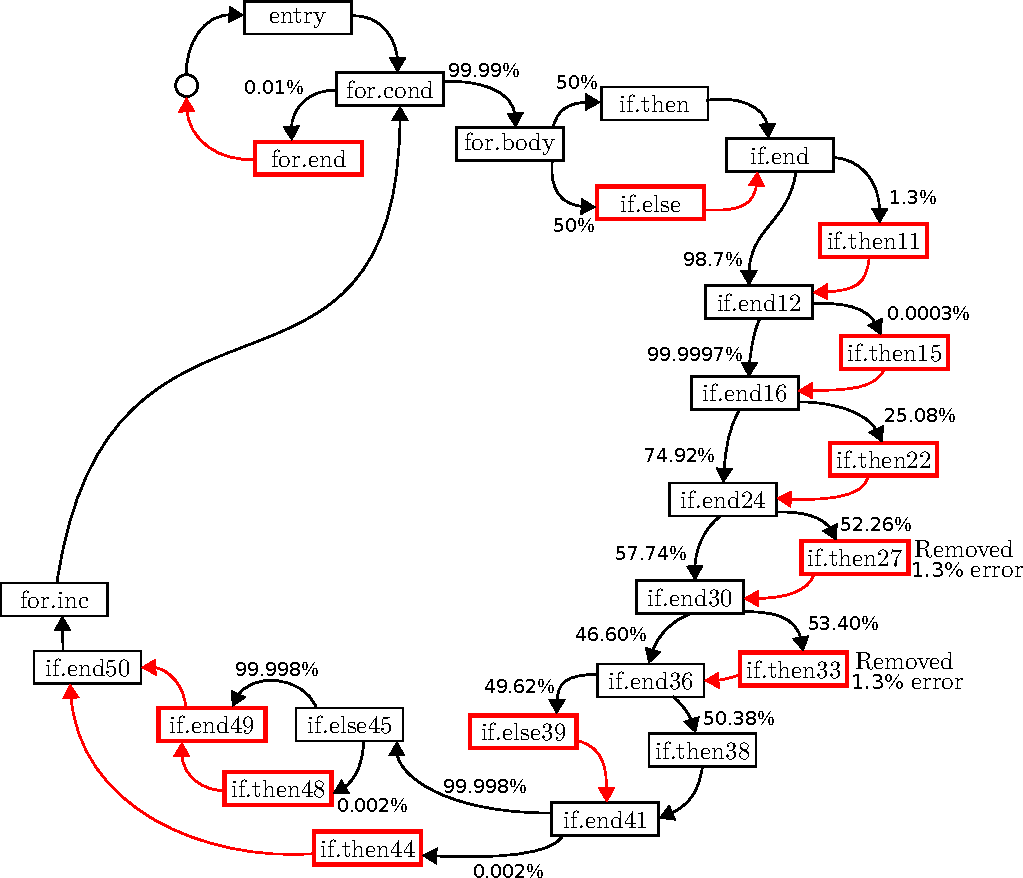
\includegraphics[width=0.395\textwidth]{figs/adpcm_d-cfg-instr.pdf}
%    \caption{CFG of the function that contains the hot loop of the {\flagstype adpcm\_d} benchmark.}
%    \label{fig:adpcm_d-cfg-instr}
%\end{figure}

The overhead for \OptProf typically remains below or around 10\% but can reach up to 59\% for \texttt{adpcm\_d}, which would be
unacceptable. \WCRelax-\textit{5}\% on the other hand manages to eliminate most of the overhead, with a worst
case of 16\% and an average of 8\%. \WPRelax-\textit{5}\% further reduces the cost of profiling, 5\% overhead on average and 13\%
worst case. For both \WCRelax and \WPRelax setting the threshold to 2\% makes it too difficult to remove probes. As a result, overhead
remain high.

\begin{figure*}[t!]
    \centering
    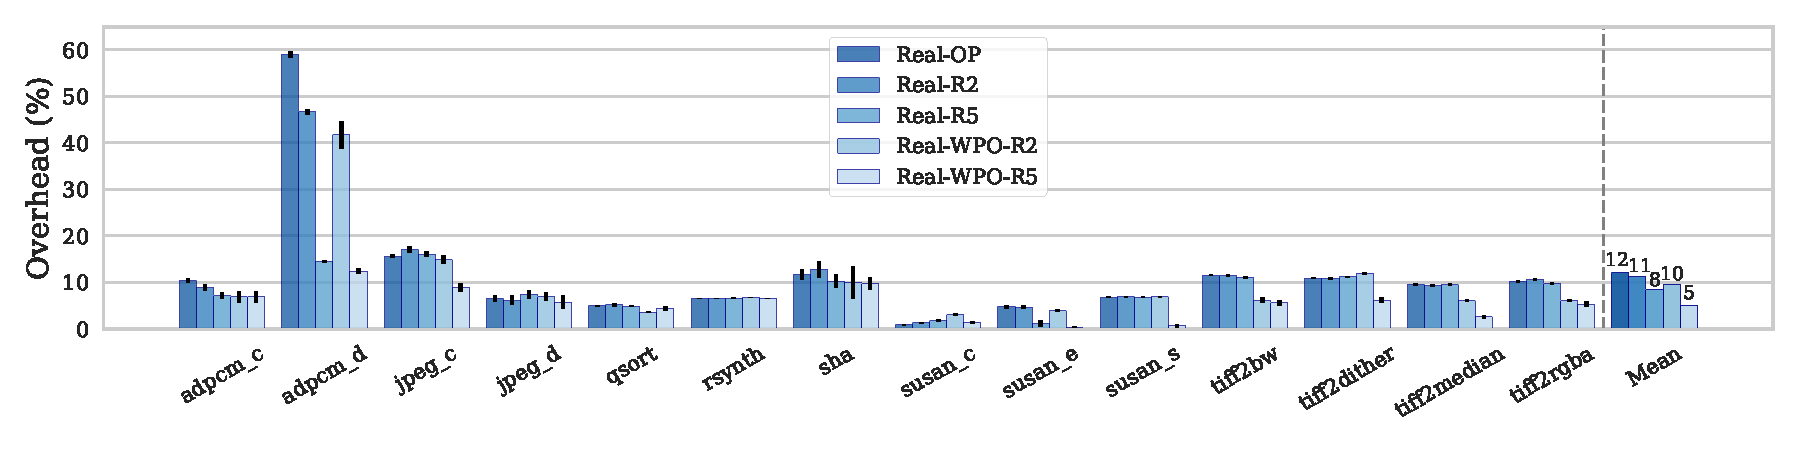
\includegraphics[width=\textwidth]{figs/overhead-O3.pdf}
    \caption{Overhead of the instrumentations compiled with {\flagstype -O3}.}
    \label{fig:overhead-O3}
\end{figure*}
\begin{figure*}[t!]
    \centering
    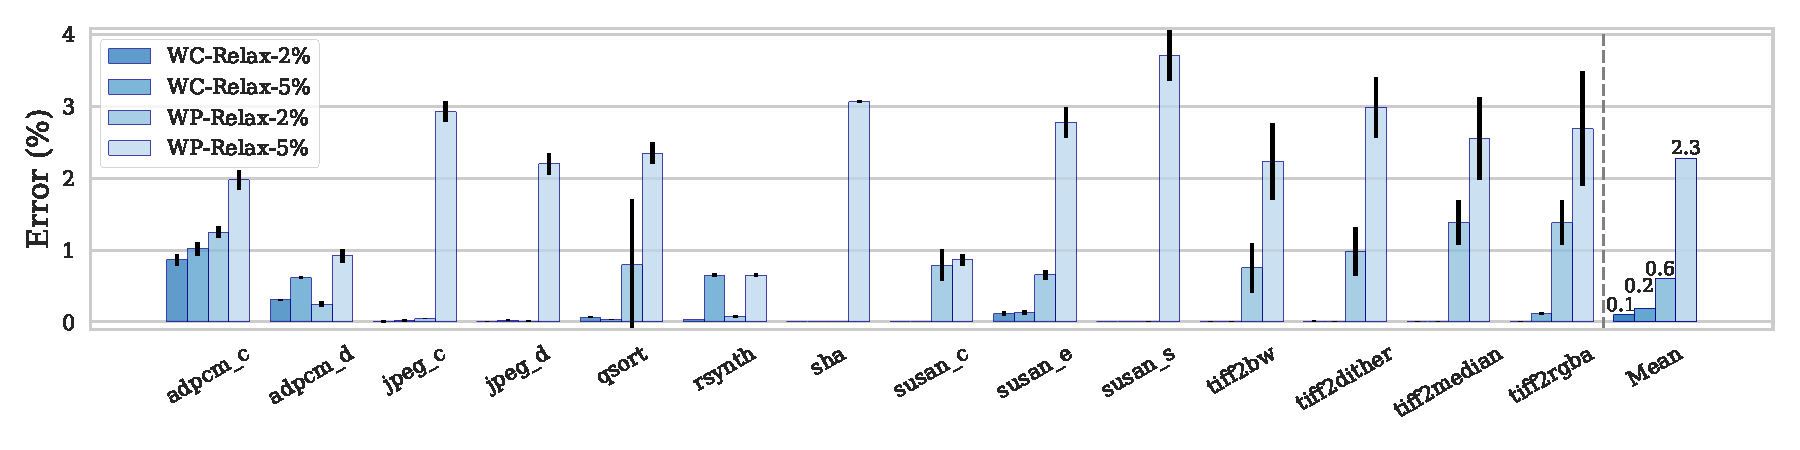
\includegraphics[width=\textwidth]{figs/error-O3.pdf}
    \caption{Dynamic error of the work profiling averaged over the 1000 inputs, after relaxing the number of probes.}
    \label{fig:error-O3}
\end{figure*}

%Mean values...
%Real-R5: 30.43\%
%WPO-R5:  54.97\%
%adpcm_d:
%Real-R5: 75.51\%
%WPO-R5:  79.07\%

The benchmark where \OptProf records its worst result, \texttt{adpcm\_d}, has a single hot function which consists mainly of a single hot
loop with several branches. This leads to numerous short basic blocks, many of them with probes. Most of the improvement achieved by both
relaxation strategies comes from removing only two probes from the hot loop. They were initially placed in branches with a high probability
of being taken but with a small work contribution. Removing either of the probes introduces error of about 1.3\% at the loop level but
eliminates three quarters of the overhead.

For a few of the benchmarks, relaxation unexpectedly introduces additional overhead. This is counter-intuitive since relaxation leads to
less computational work. In these cases, relaxation did not manage to remove high frequency probes, so we did not benefit significantly.
On the other, the probes that were removed affected how \texttt{-O3} optimized the surrounding code, in some cases blocking useful
optimizations that were applied originally. This resulted in slower code.
%For example, some of the optimizations that make use of this built-in cost model
%and also alter the CFG are: loop-unrolling, function inlining, and
%simplifications of the CFG.
%These changes in the program's CFGs may affect other compiler optimizations and
%also possibly in hardware performance, for example affecting the instruction
%caching.

In Figure~\ref{fig:error-O3}, we see the error in our work estimation introduced by relaxation. The error for the WC-Relax strategies is
too low, always below 1\% and usually much lower, regardless of threshold. This confirms that WC-Relax is too conservative. WP-Relax brings
us closer to our target threshold. Despite not having hard guarantees for the error under WP-Relax, in all cases the error was below the
threshold.

\subsection{Evaluation of Online {\IterComp}}

\begin{figure*}[t]
    \centering
    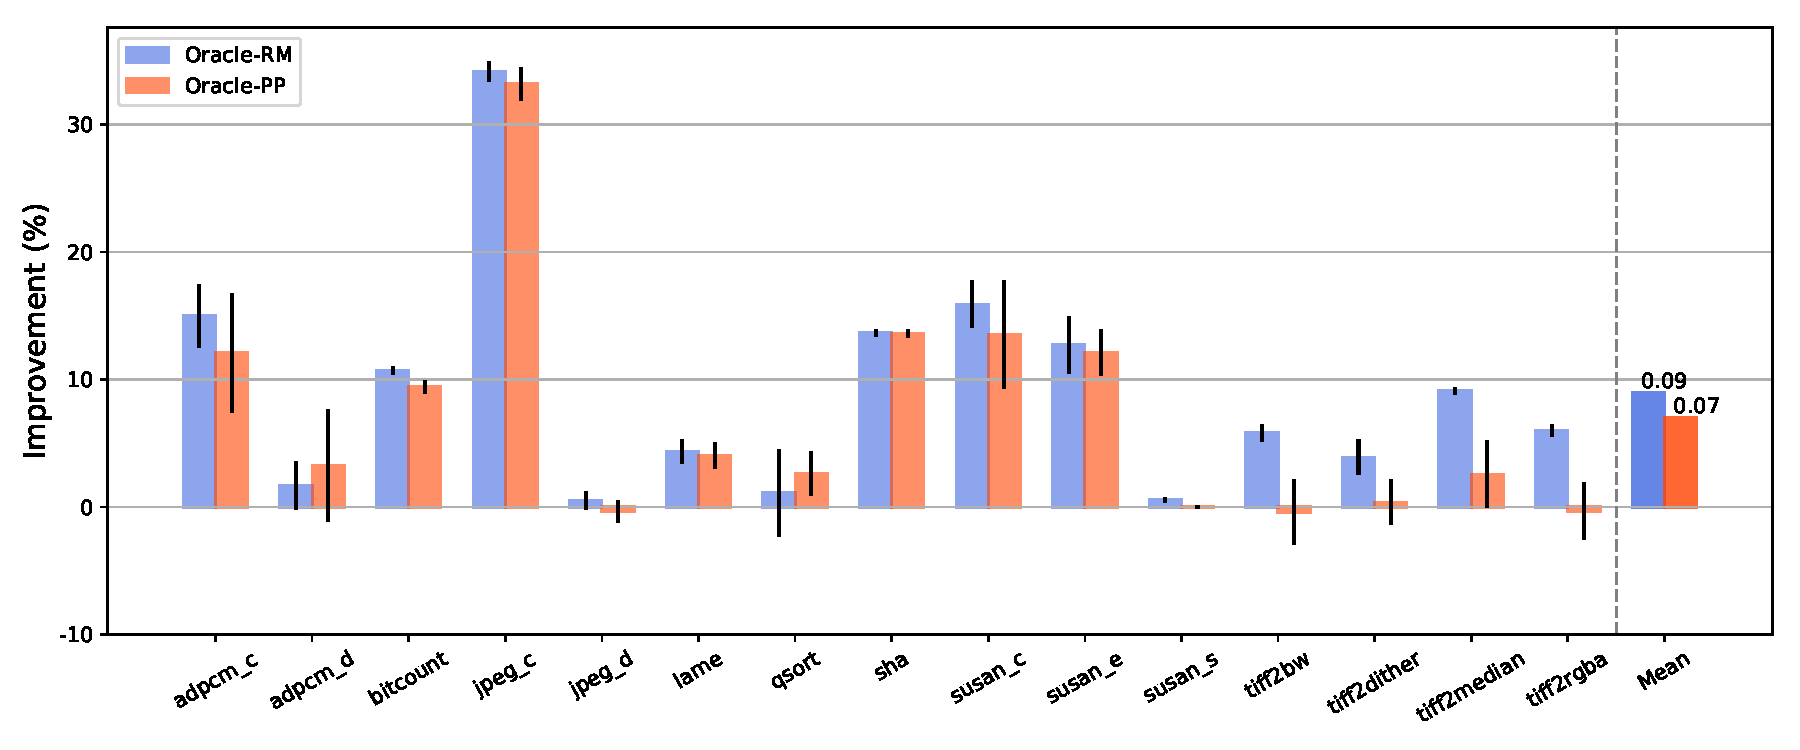
\includegraphics[width=\textwidth]{figs/speedups.pdf}
    \caption{Speedups obtained from the final optimization sequence selected by the online {\itercomp}.
	         The speedups reported for each benchmark represents the average speedup across their complete 1000 input datasets.}
    \label{fig:speedups}
\end{figure*}

In this section we evaluate the effectiveness of our work efficiency metric.
We perform online {\itercomp} using all five profiling strategies, namely
\OracleRM, \OraclePP,\OptProf,\WCRelax-5\%, and \WPRelax-5\%.
Because the \OracleRM measures actual speedup, it provides reference results for
assessing the effectiveness of the work-efficiency metric.
For the relaxation strategies, we evaluate only those with a 5\% threshold, since
they offered better overhead reductions for little dynamic errors in the measurement.

For all strategies, the same optimization sequence is used for multiple inputs, using a dynamic input-window size, as explained in
Section~\ref{sec:oic-infra}. The average performance over the input window provides an estimate for the overall performance of the
optimization sequence across distinct inputs. The optimization sequences are ranked based on their average performance, and the best
optimization sequence is selected.

The comparison between \OracleRM and \OraclePP is crucial for validating the
effectiveness of the work efficiency metric in guiding online {\itercomp},
while the other configurations demonstrate the viability of applying online
{\itercomp} in real-world scenarios.

In order to evaluate the quality of the final optimization sequences selected by each configuration of the online {\itercomp}, we compare
their speedup over the \texttt{-O3} optimization across all the 1,000 inputs of the benchmark being optimized. None of the configurations
degrades the performance over \texttt{-O3} (with statistical significance).
%When measuring the wall-clock time for each input, to reduce noise, we execute
%the same input until we have a statistically sound measurement, i.e. we execute
%until we have an interval no larger than 1\% with 99\% confidence.
Figure~\ref{fig:speedups} shows these average speedups for all test benchmarks.
This figure shows that the best optimization sequence selected with the Oracle-PP
is very close to the performance of the best optimization sequence selected with
the \OracleRM, where \OraclePP achieves on average about 80\% of the performance
improvement obtained by the \OracleRM.
This result is important for demonstrating that our work efficiency metric has
the potential to produce good results in real-world online scenarios.

The \OptProf achieves 4\% improvement on average, which represents 45\% of the
performance improvement obtained by the \OracleRM.
This difference to \OraclePP is explained by the real (intrusive) profiling used
in the \OptProf configuration.
The profiling affects the search in two key ways:
\textit{(i.)} the overhead incurred by the profiling affects the execution time,
and therefore also affects the work efficiency metric,
\textit{(ii.)} the instrumentation code may affect many of the optimizations, e.g.,
due to the use of a global variable or in decisions taken based on a cost-model
for the instructions.
However, even in the \OptProf configuration, which has a highly intrusive instrumentation,
it is still possible to obtain performance improvements in a realistic online
{\itercomp}.

Finally, the evaluation also indicates that the use of relaxation algorithms
is beneficial not only for its reduction in overhead, which is directly observed
by the user, by it also tends to improve the quality of the search.
This improvement has to do with the aforementioned effects of an intrusive
instrumentation on the search.
The relaxation has the potential to reduce both effects of the profiling.
Both the \WCRelax-5\% and \WPRelax-5\% achieve about 60\% of the
performance improvement obtained by the \OracleRM.
